\documentclass[12pt,a4]{article}




\usepackage{graphicx,amsmath,amssymb,amsthm, boxedminipage,xcolor}

%\usepackage[lined,boxed]{algorithm2e}

\usepackage{algorithm}
\usepackage{algpseudocode}

%\usepackage{algorithmic}
\usepackage{algpseudocode}
\usepackage{amsmath}
\usepackage{graphics}
\usepackage{epsfig}

\newtheorem{theorem}{Theorem}[section]
\newtheorem{proposition}[theorem]{Proposition}
\newtheorem{lemma}[theorem]{Lemma}
\newtheorem{corollary}[theorem]{Corollary}
\newtheorem{definition}[theorem]{Definition}

\newtheorem*{theorem*}{Theorem}
\newtheorem*{lemma*}{Lemma}
\newtheorem*{proposition*}{Proposition}


\newtheorem{exercise}[theorem]{Exercise}
\newtheorem{exerciseD}[theorem]{*Exercise}
\newtheorem{exerciseDD}[theorem]{**Exercise}

\let\oldexercise\exercise
\renewcommand{\exercise}{\oldexercise\normalfont}

%\let\oldexerciseD\exerciseD
%\renewcommand{\exerciseD}{\oldexerciseD\normalfont}

%\let\oldexerciseDD\exerciseDD
%\renewcommand{\exerciseDD}{\oldexerciseDD\normalfont}

\newcommand{\E}{\mathbb{E}}
%\newcommand{\nth}[1]{#1^{\textsuperscript{th}}}
\newcommand{\scalar}[2]{\ensuremath{\langle #1, #2\rangle}}
\newcommand{\floor}[1]{\left\lfloor #1 \right\rfloor}
\newcommand{\ceil}[1]{\left\lceil #1 \right\rceil}
\newcommand{\norm}[1]{\|#1\|}
\newcommand{\pfrac}[2]{\left(\frac{#1}{#2}\right)}
\newcommand{\nth}[1]{#1^{\textsuperscript{th}}}
\newcommand{\core}{\textnormal{core}}



\newif\ifsolution

\solutionfalse

\newcommand{\answer}[1]{
\ifsolution
{\color{blue} #1}
\else
\fi
}



\newcommand{\poly}{\textnormal{poly}}
\newcommand{\quasipol}{\textnormal{quasipol}}
\newcommand{\ssubexp}{\textnormal{stronglySubExp}}
\newcommand{\wsubexp}{\textnormal{weaklySubExp}}
\newcommand{\simplyexp}{\textnormal{E}}
\newcommand{\expo}{\textnormal{Exp}}



\newcommand{\N}{\mathbb{N}}
\newcommand{\nn}{\mathbb{N}_0^n}
\newcommand{\R}{\mathbb{R}}
\newcommand{\Z}{\mathbb{Z}}


\definecolor{darkgreen}{rgb}{0,0.6,0}


\date{}

\title{
  Mathematical Foundations \\of \\Computer Science\\
  \vspace{3mm}
{\normalsize CS 499,	Shanghai Jiaotong University,  Dominik Scheder}
}

\begin{document}

\maketitle

%\begin{quotation}
%  You are welcome to discuss the exercises in the discussion
%  forum. Please take them serious. Doing the exercises is as important
%  than watching the videos.
%
%  I intentionally included very challenging exercises and marked them
%  with one or two ``$*$''. No star means you should be able to solve
%  the exercises without big problems once you have understood
%  the material from the video lecture. One star means it requires 
%  significant additional thinking. Two stars means it is not 
%  unlikely that you will fail to solve them, even once you have understood
%  the material and thought a lot about the exercise. Don't feel bad
%  if you fail. Failure is part of learning.
%
%  This is the first time this course is online. Thus there might be mistakes
%  (typos or more serious conceptual mistakes) in the exercises. I will be 
%  grateful if you point them out to me!
%\end{quotation}





\setcounter{section}{8}

\section{Hamilton Cycles, Hamilton Paths, and Non-isomorphic Trees}



\begin{itemize}
 \item Homework assignment published on Monday 2018-04-23
 \item Submit your first solution by Sunday, 2018-04-29, 18:00, by email
 \item Submit your final solution by Sunday, 2018-05-06.
\end{itemize}

\subsection{Regular Orientations of a Regular Graph}

We call a graph {\em $d$-regular} if every vertex has degree $d$.
A directed graph is $(d,d)$-regular if every vertex has $d$ incoming and $d$
outgoing edges.

\begin{exercise}
   Show that in every $4$-regular graph, you can orient the edges such that every vertex
   has two incoming and two outgoing edges, i.e., such that the resulting
   digraph is $(2,2)$-regular. See the picture below for an illustration.
\end{exercise}
\begin{center}
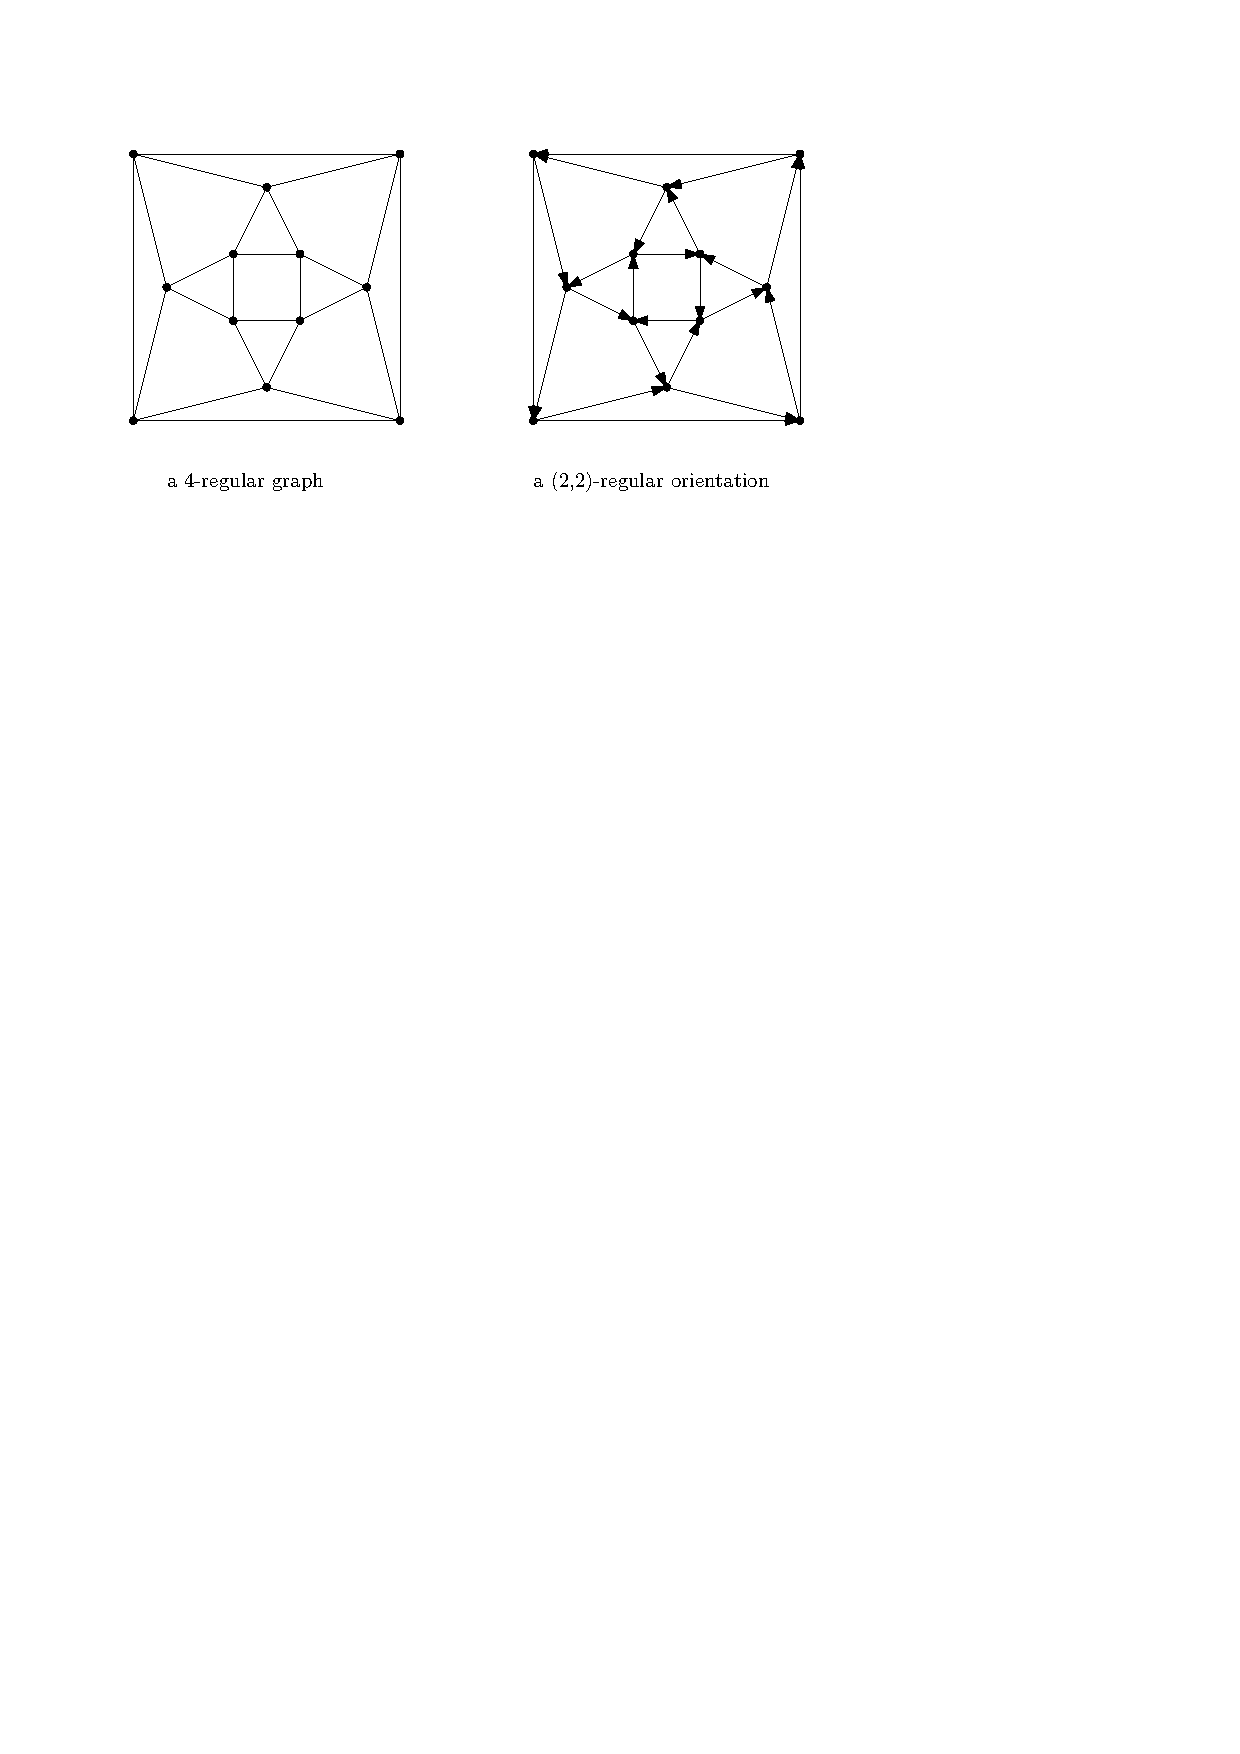
\includegraphics[width=\textwidth]{figures/four-regular-oriented.pdf}
\end{center}
\textbf{Solution.}
Since the degree of each vertex in the graph is even, there must be an Euler circuit in the graph. The direction of the edge is oriented along the Euler loop. For any vertex, if there is an edge entering it, there must be another edge to leave it. A vertex with a degree of 4 means that it has two incoming and two outgoing edges.




\subsection{Hamilton Cycles and Ore's Theorem}

Consider $K_n$, the complete graph on $n$ vertices. For $n \geq 3$, this obviously has a Hamilton cycle.
How many edges do you have to delete from $K_n$ to destroy all Hamilton cycles? That is, what is the
smallest set $S$ such that $\left( V, {V \choose 2} \setminus S\right)$ has no Hamilton cycle? Let $s_n$ denote
the size of this set (this depends on $n$, thus the notation $s_n$). For example, $s_2 = 0$ since $K_2$
has no Hamilton path to begin with; $s_3 = 1$ since removing one edge from $K_3$ results in a graph without
a Hamilton cycle.

\begin{exercise}
 Find a closed formula for $s_n$ and prove it! \textbf{Hint.} One part will be easy. For the other part,
 use Ore's Theorem.
\end{exercise}

\textbf{Solution.}
\[s_n = n-2\]
\qquad In a complete graph, the degree of each point is n-1. We can remove the n-2 edges connected to the same point v, so that only one edge is connected to v. It is impossible to form a loop in the graph, not to mention Hamilton circuit.\par
\quad What if we only delete n-3 edges? $\forall u,v \in V,u\neq v$,$l_u$ and $l_v$ is the number of degrees that the u and v lose after deleting n-3 edges.The best case is that the deleted edges are all connected to u or v and include (u, v), which means that $l_u + l_v \le 2 + (n-4) = n-2$. So $d(u)+d(v)=2*(n-1)-(l_u+l_v)\ge n$. According to the Ore's Theorem, there exits a Hamilton circuit in the graph.

\begin{center}
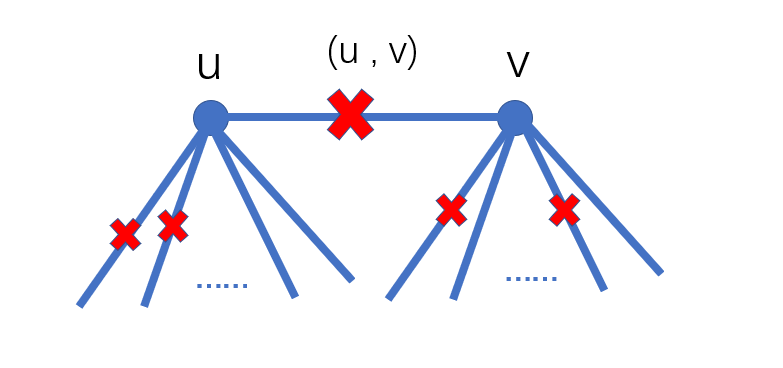
\includegraphics[scale=0.6]{2.png}
\end{center}

A {\em tournament} is a directed graph in which, for each pair $u,v \in V$, exactly one of the
directed edges $(u,v)$ and $(v,u)$ is in the graph. Imagine a sports tournament in which every participant
plays against every other exactly once. Draw an arc from $u$ to $v$ if $u$ beat $v$ in this tournament.

\begin{center}
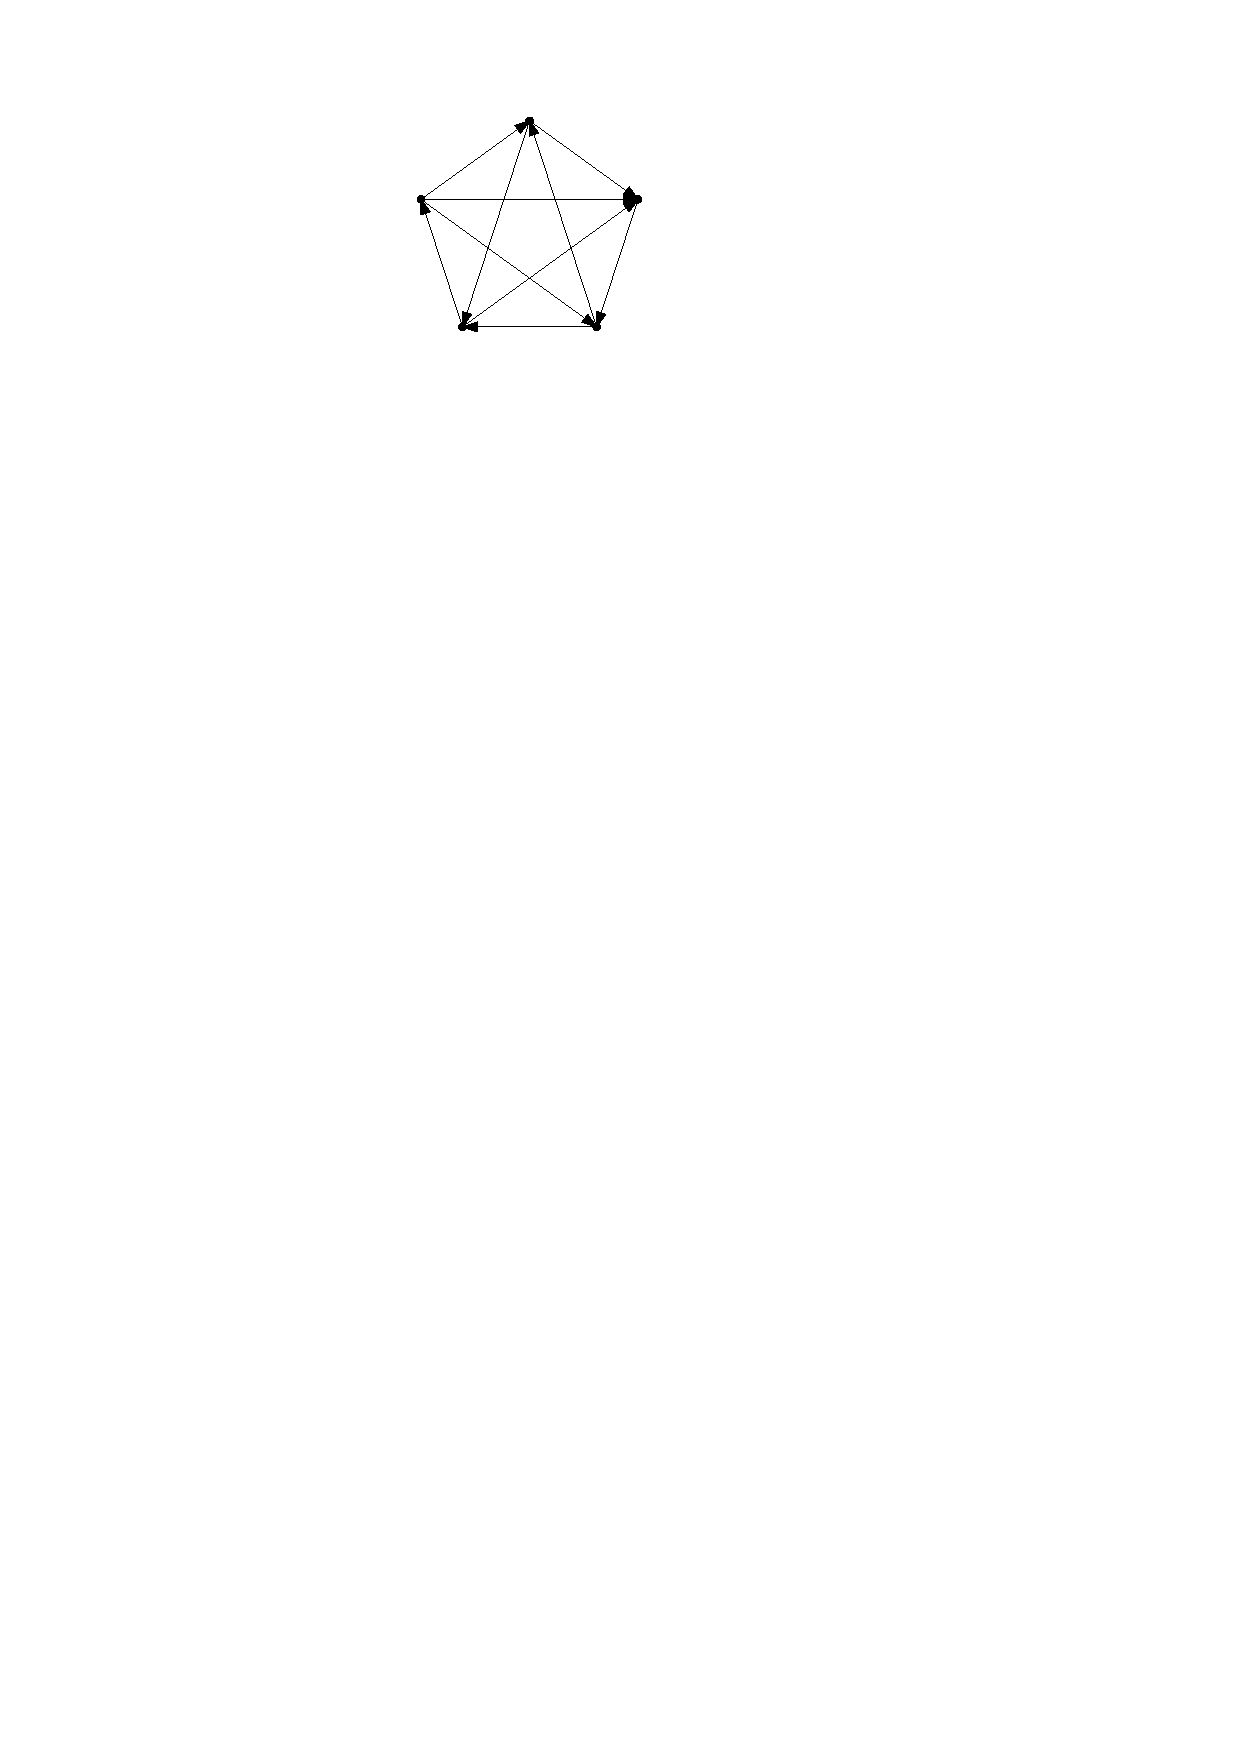
\includegraphics[width=0.5\textwidth]{figures/tournament-five.pdf}\\
{\small A tournament on five vertices.}
\end{center}

\begin{exercise}
   Show that every tournament has a {\em directed Hamilton path}, i.e., a sequence
   $u_1,u_2,\dots,u_n$ such that $(u_i, u_{i+1}) \in E$ for all $i = 1,\dots, n-1$. See the picture below.

\begin{center}
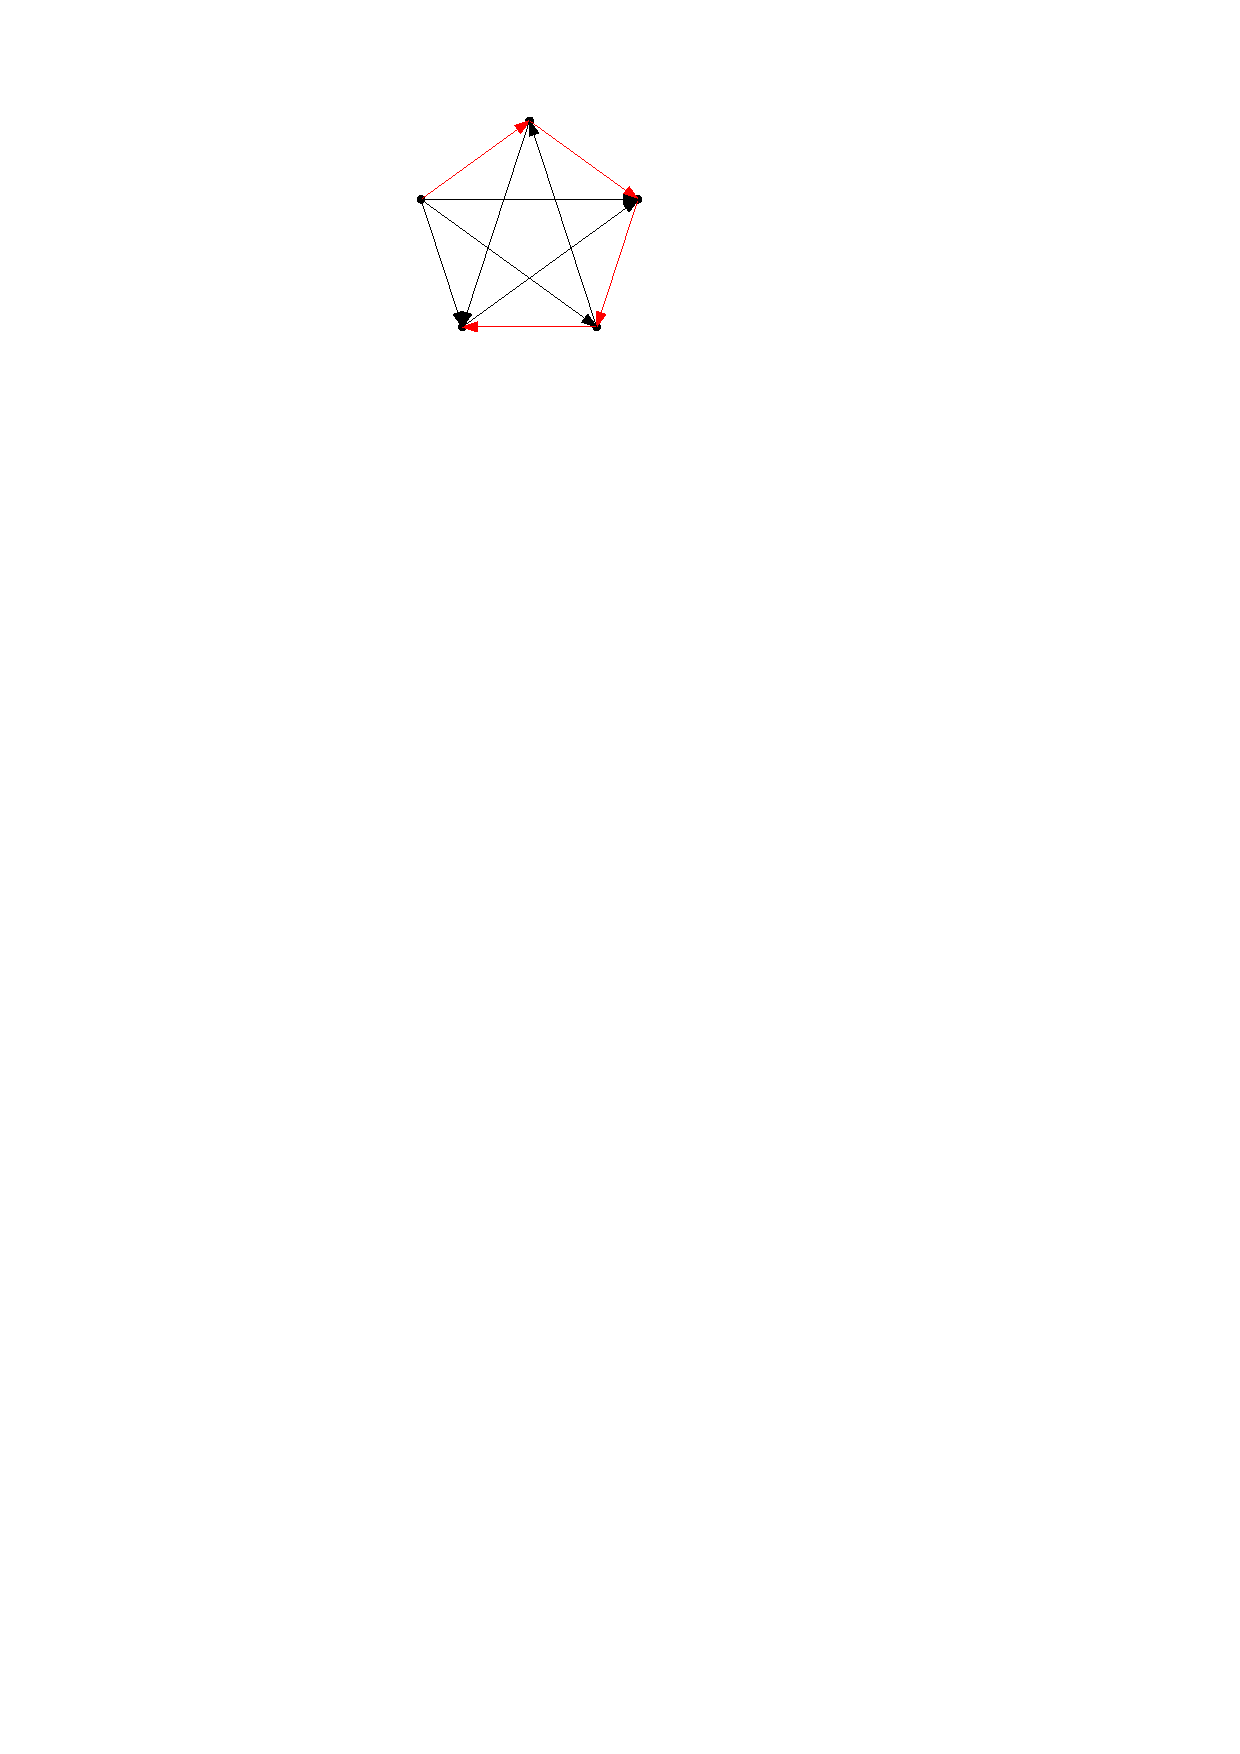
\includegraphics[width=0.5\textwidth]{figures/tournament-five-path.pdf}\\
{\small The same tournament with a Hamilton path.}
\end{center}
  You probably won't be able to use the proof of Ore's Theorem directly, but you can use the proof idea.
\end{exercise}
\textbf{Proof.}
\par We prove it by contradiction. 
\par We assume that the longest  directed Hamilton Path has $k(k<n)$ vertices for a tournament with $n$ vertices. Let $x$ be a vertex not in the path. As is shown in the graph, the $2$ edges between $(1,x)$ and $(k,x)$ must be $1 \rightarrow x$ and $x \rightarrow k$, otherwise, why not we add $x$ into the path ,making the path longer? If so, because the edge between $(1,x)$ and $(k,x)$ have different direction with regard to $x$. So we can infer that no matter what the direction between $(x,i)(2\le i\le k-1)$ is, there must be an $i(1\le i\le k-1)$ such that there is path from $1\rightarrow2\rightarrow\cdots\rightarrow i\rightarrow x\rightarrow i+1\rightarrow k-1\rightarrow k$, which is longer that the path we assume before. There is a contradiction, so the statement holds.
\begin{center}
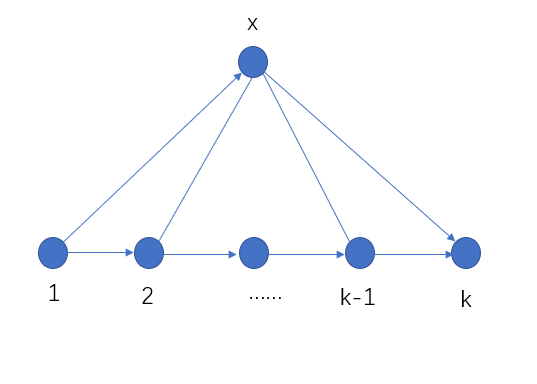
\includegraphics[width=0.5\textwidth]{lym1.PNG}
\end{center}

\subsection{Isomorphism Classes of Trees}

In the lecture (and in the videos) we have seen that the number of trees on
vertex set $V = \{1,2,\dots,n\}$ is $n^{n-2}$. This however ignores isomorphisms.
For example, there are $3^{3-2} = 3$ trees on vertex set $\{1,2,3\}$, but all those
trees look alike (are isomorphic). On $\{1,2,3,4\}$, there are 16 trees, but
there are only two isomorphism classes: the path and the star. For five vertices, there are 125 trees
but only three isomorphism classes: the path, the star, and the ``T-shape'' (see video on
counting the number of trees). For $n=6$ we get the path, the Y-shape, the Euro symbol, the Star Wars fighter, the Scandinavian cross, and the star, so six isomorphism classes (but a total of 1296 trees).

\begin{exercise}
  List of isomorphism classes on seven vertices. That is, draw trees $T_1,\dots,T_m$ on seven vertices such that
  no two of them are isomorphic but every tree on seven vertices is isomorphic to one of them.
  How many do you get?
\end{exercise}



\begin{tabular}{r|c|c|c|c|c|c|c}
$n$ & 1 & 2 & 3 & 4 & 5 & 6 & 7 \\ \hline
number of isomorphism classes &
          1 & 1 & 1 & 2 & 3 & 6 & 11
\end{tabular}
\vspace{5mm}

Alright, so let's denote by $t_n$ the number of isomorphism classes of trees on $n$ vertices.
That is, $t_n$ is the largest number $m$ such that we can find trees $T_1,\dots,T_m$ on
$n$ vertices such that no two of them are isomorphic. We would like to have an exact and
 explicit formula for $t_n$, but that is probably too much to ask for.
Instead, let us try to understand $t_n$ approximately and asymptotically.

\begin{exercise}
  Show that $t_n \leq 4^n$. Hint: Consider the video on the isomorphism problem on trees.
  It defines a way to encode a tree as a $0/1$-sequence.
\end{exercise}
\textbf{Solution.}
From the way to encode a tree as a $0/1$-sequence, we can know that there is totally $2n$ bits in the sequence, with every bit having $2$ choices: $0$ and $1$. So there are totally $2^{2n}=4^n$ sequences. Obviously, $t_n \leq 4^n$.

\begin{exercise}
  Show that $t_n \geq \frac{e^n}{\poly(n)}$, where $\poly(n)$ is some polynomial in $n$.
  Hint: There are $n^{n-2}$ trees on $V = [n]$. We group them together in ``buckets''
  of isomorphic trees. How large can a bucket be? Answer this and then use Stirling's approximation
  for $n!$.
\end{exercise}

\begin{exerciseDD}
   Try to improve those bounds. That is, find some $a < 4$ such that $t_n \in O(a^n)$ or
   some $b > e$ such that $t_n \in \Omega(b^n)$. Any improvement will be kind of interesting.
   Aim for simple proofs!
\end{exerciseDD}

\textbf{Remark.} The ``true'' rate of growth is known by a result of George P\'olya but apparently
it is quite difficult (I write ``apparently'' because I have never studied this work).


\end{document}
